
\documentclass[10pt,a4paper,english]{article}

\usepackage[margin=2.5cm]{geometry}
\addtolength{\textheight}{-1cm}

\usepackage{bold-extra}
\usepackage{listings}
\lstset{
basicstyle=\ttfamily,
numbers=left,
numberstyle=\footnotesize,
frame=single,
tabsize=4,
breaklines=true,
breakatwhitespace=true
}

\usepackage{enumerate}
\usepackage{graphicx}
\usepackage{fancyhdr}
\usepackage{amsmath}
\usepackage{diagbox}
\usepackage{subfig}
\pagestyle{fancy}

\setlength{\headheight}{40pt} 
\lhead{Sebastien Duc (186935) \\* Yann Schoenenberger (186768)}
\rhead{Pattern Classification and Machine Learning \\* \today}

\begin{document}

\begin{center}
\huge{\textbf{PCML Miniproject}}
\end{center}

\section*{Introduction}

The aim of this project was to gain practical experience in machine learning by writing and testing software that differentiates between hand-written digits.
To do that, we implemented two different methods: Multi-Layer Perceptron (MLP) and Support Vector Machines (SVM). To use those, we also had to take care of preprocessing and splitting the available samples into training, validation and test sets. Also, we had to experiment with and compare various arbitrary constants we have to choose in both methods and see how these choices impact the accuracy and efficiency of the classification.

\section*{Multi-Layer Perceptron}

\subsection*{Splitting and Preprocessing}

We are given 6000 patterns and we keep two thirds of them (i.e. 4000) in our training set and the rest (i.e. 2000) in our validation set. Before the split, the collection of vectors is shuffled so that we break any potential ordering of the vectors that may bias our classification.\\*
The preprocessing is very simple since the MNIST data is already very clean and usable. We simply normalize all vectors $ v $ by dividing all elements of $ v $ by $ v $'s largest element.

\subsection*{MLP Setup}

Let us first describe how we built the MLP.
First of all we had to derive some formula so that we could compute the gradient.
From the course notes, we have that
\[
    \begin{split}
        \nabla_{\bf w^{(2)}}E_i = r^{(2)} {\bf z^{(1)}} \quad,\quad \frac{\partial E_i}{\partial b^{(2)}}  = r^{(2)}\\
 \nabla_{\bf w_q^{(1)}}E_i = r_q^{(2)} {\bf x} \quad, \quad \frac{\partial E_i}{\partial b_q^{(1)}}  = r_q^{(1)}\\
    \end{split}
\]
The residuals are the following in our case:
\[
        r^{(2)} = \frac{-t_i e^{-t_i a^{(2)}}}{1 + e^{-t_i a^{(2)}}}
\]
\[
        r_q^{(1)} = \left\{
            \begin{array}{l l}
                r^{(2)} w_k^{(2)}\frac{a_{q-1}^{(1)} e^{-a_{q}^{(1)}}}{\left(1+e^{-a_{q}^{(1)}}\right)^2} & \quad\mbox{when } q = 2k\\
                r^{(2)} w_k^{(2)}\frac{1}{1 + e^{-a_{q+1}^{(1)}}} & \quad\mbox{when } q = 2k-1.\\
        \end{array}\right.
\]
Thus in our code, to compute the residuals of the hidden layer, we had to distinguish two cases. When it is an odd or an even hidden unit.

In the analysis we only considered a MLP with one hidden layer. We variated $h_1$ (which is the number of hidden units) from 10 to 100 by step of 10.
In Figure~\ref{fig:hidden}, you can see the $E_{\mathrm{Log}}$ for the validation set in green and for the training set in blue. We also plotted the
zero-one error in red for the validation set.
\begin{figure}[!h]
    \centering
    \subfloat[for $\eta = 0.01$  and $h_1 = 10$]{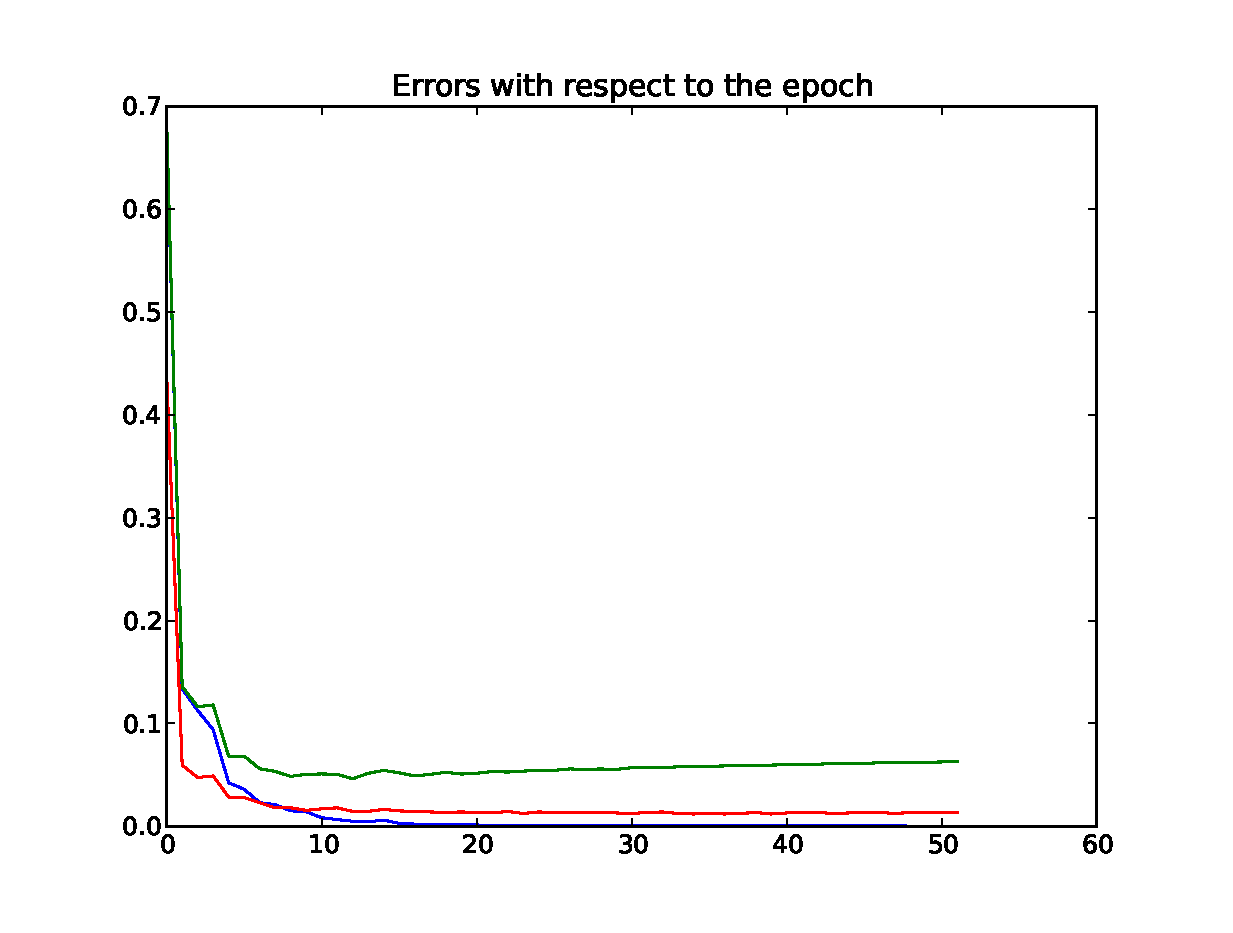
\includegraphics[width=0.3\textwidth]{../plots/learning_0.01__hidden_10.eps}}
    \subfloat[for $\eta = 0.01$  and $h_1 = 20$]{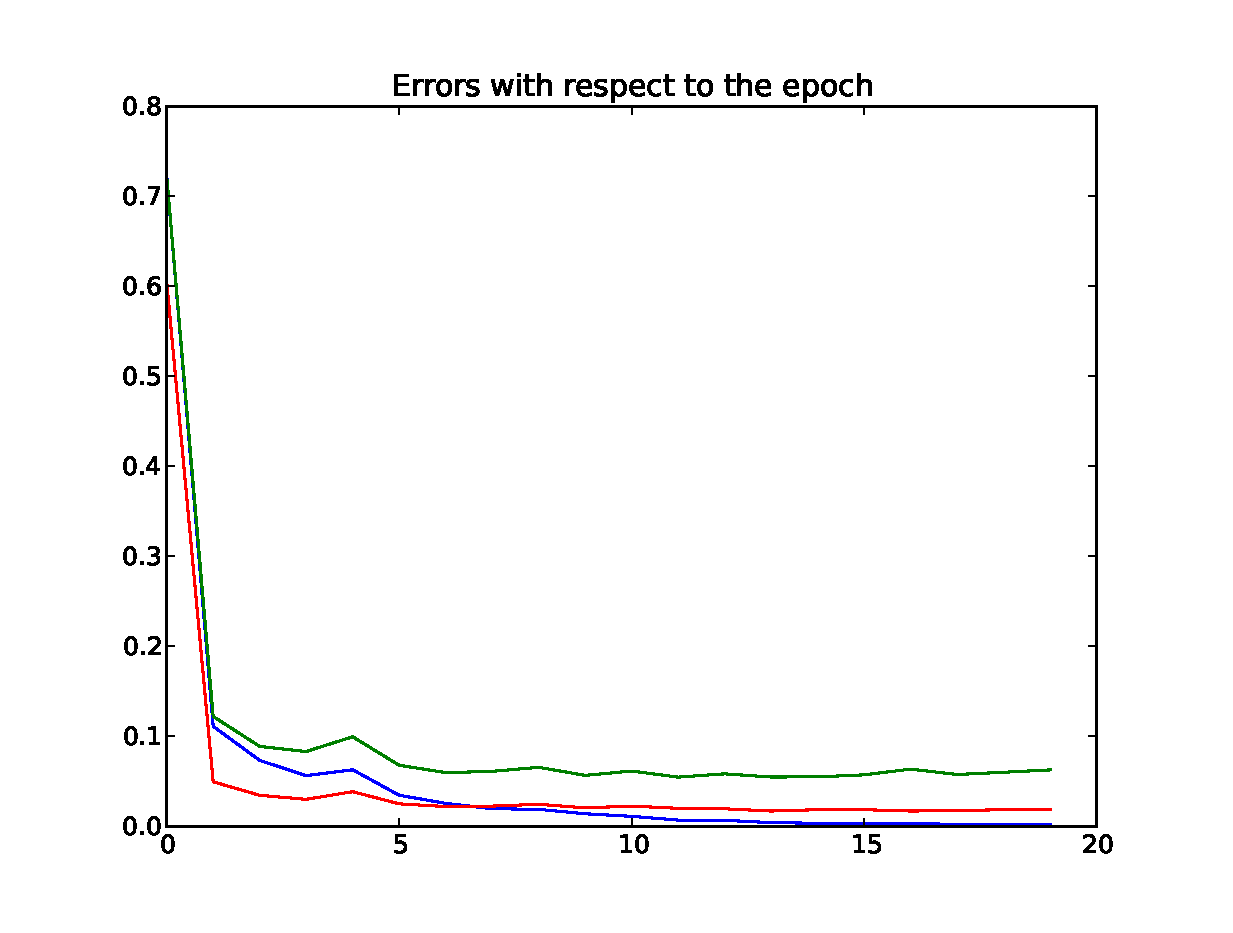
\includegraphics[width=0.3\textwidth]{../plots/learning_0.01__hidden_20.eps}}
    \subfloat[for $\eta = 0.01$  and $h_1 = 30$]{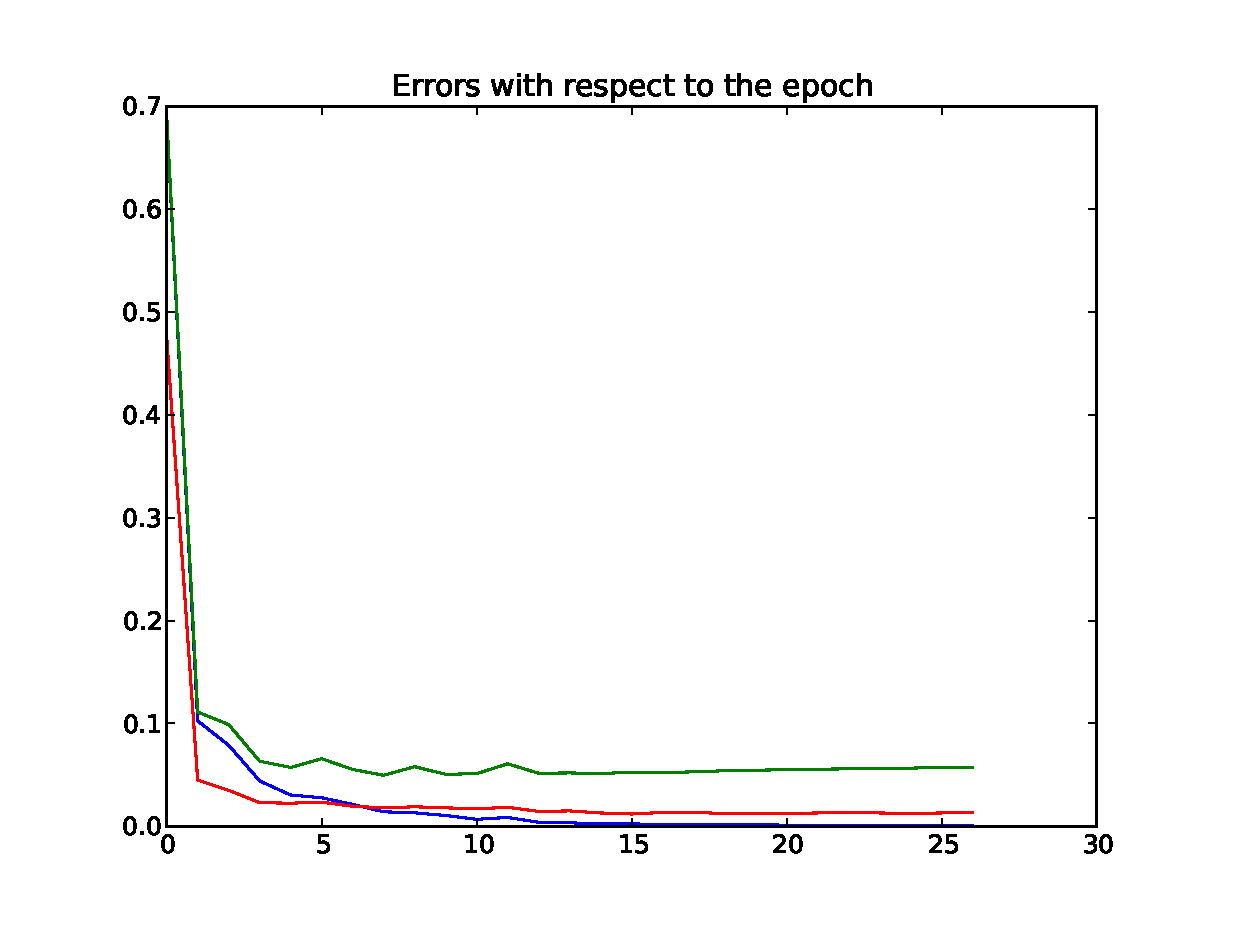
\includegraphics[width=0.3\textwidth]{../plots/learning_0.01__hidden_30.eps}}\\
    \subfloat[for $\eta = 0.01$  and $h_1 = 40$]{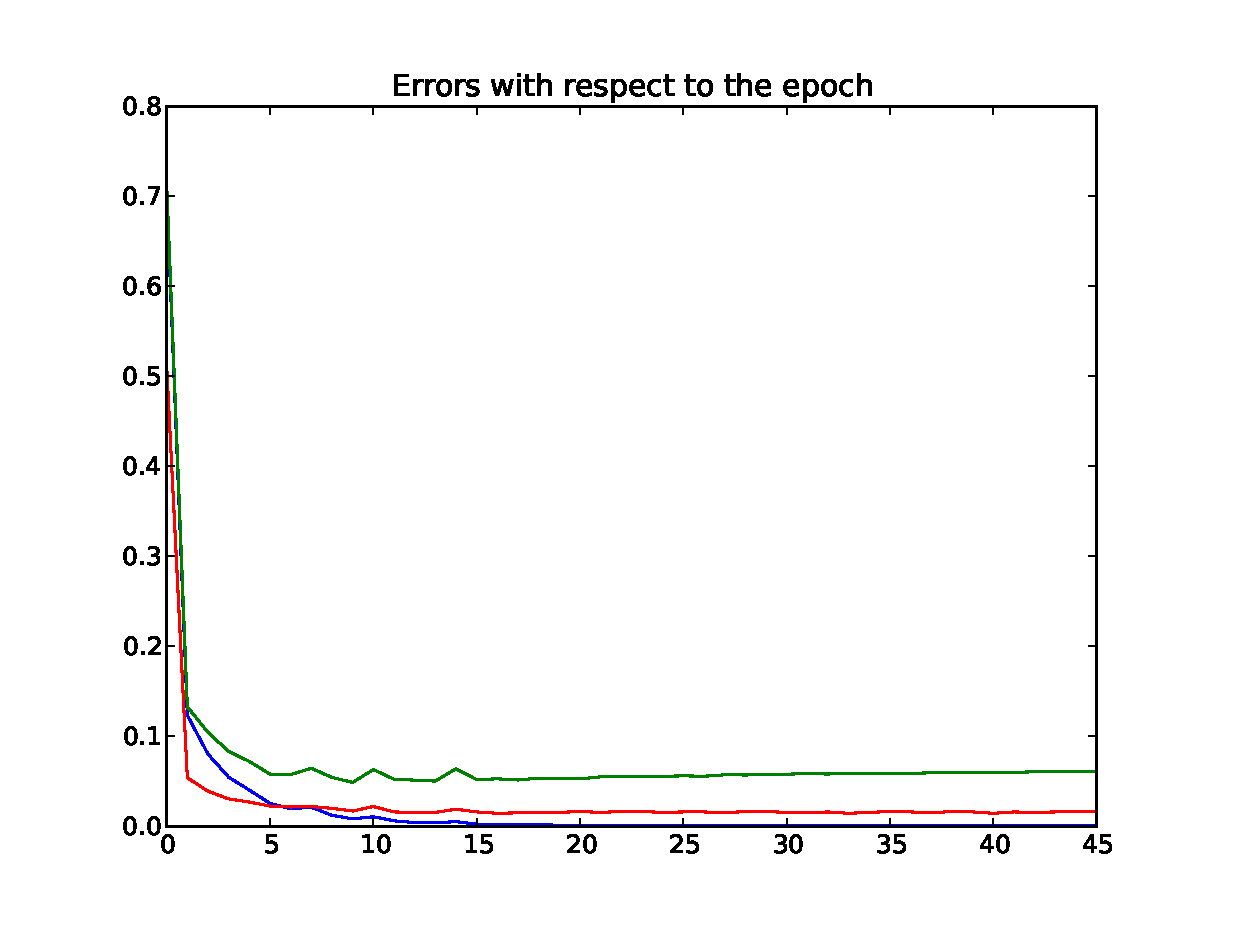
\includegraphics[width=0.3\textwidth]{../plots/learning_0.01__hidden_40.eps}}
    \subfloat[for $\eta = 0.01$  and $h_1 = 50$]{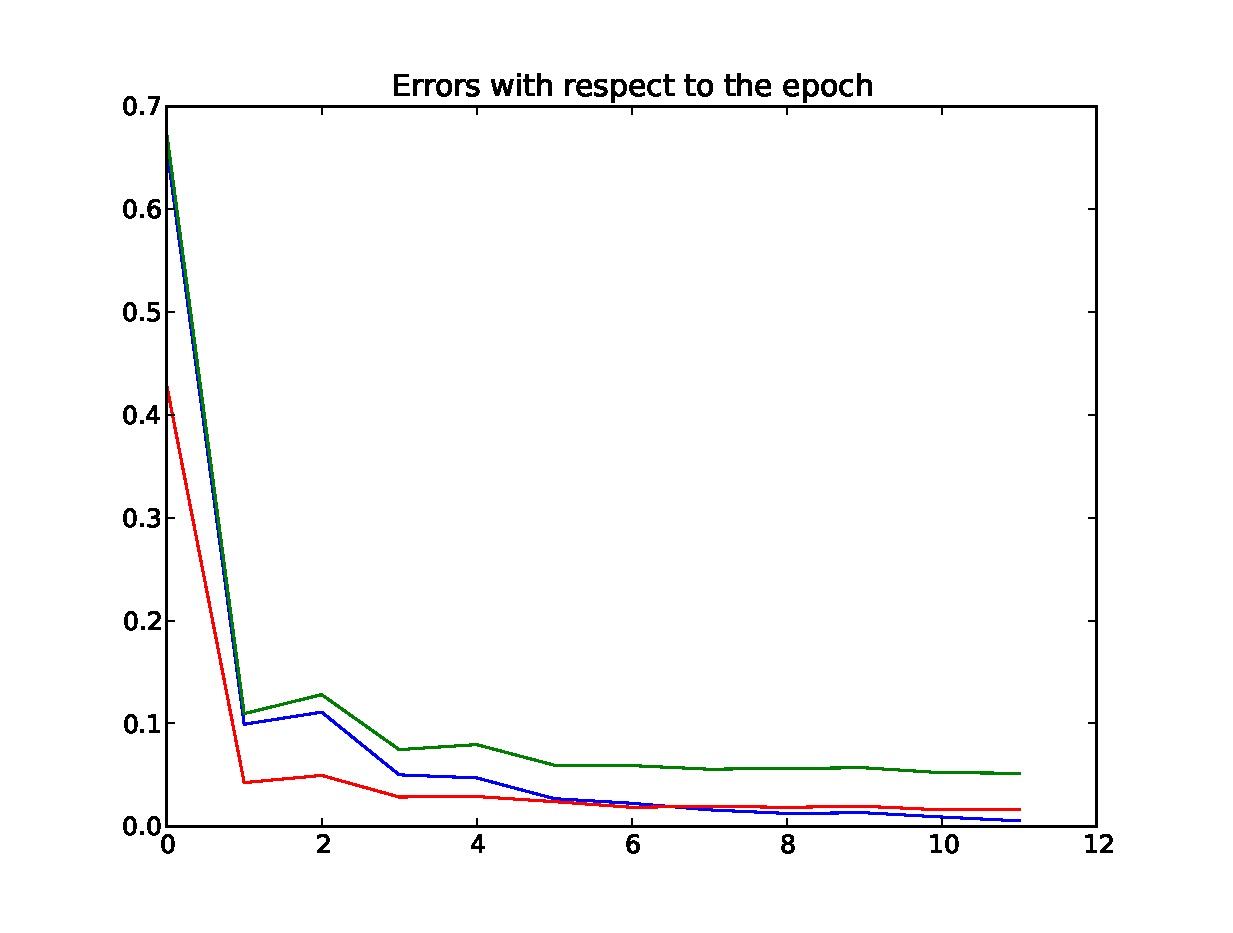
\includegraphics[width=0.3\textwidth]{../plots/learning_0.01__hidden_50.eps}}
    \subfloat[for $\eta = 0.01$  and $h_1 = 60$]{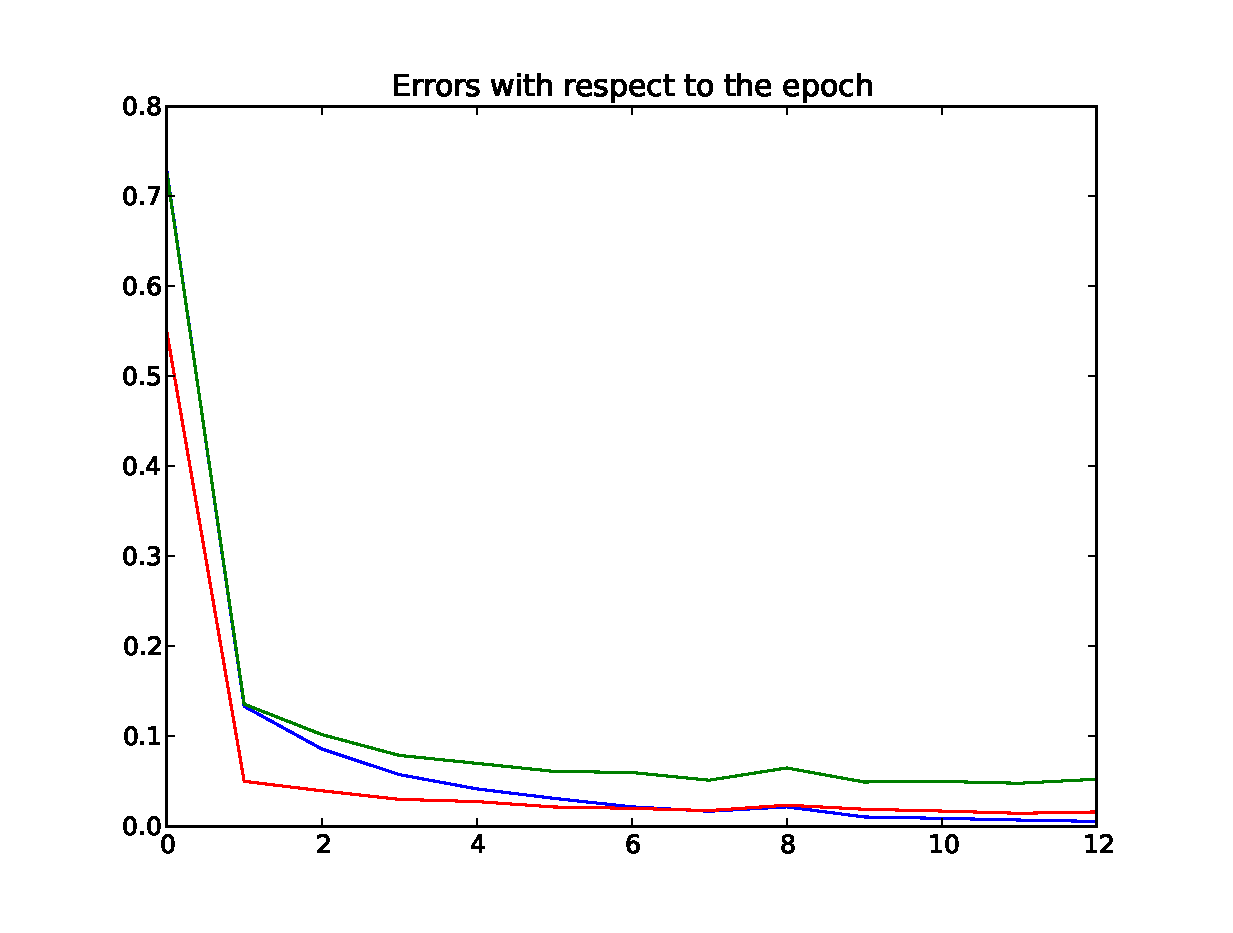
\includegraphics[width=0.3\textwidth]{../plots/learning_0.01__hidden_60.eps}}\\
    \subfloat[for $\eta = 0.01$  and $h_1 = 70$]{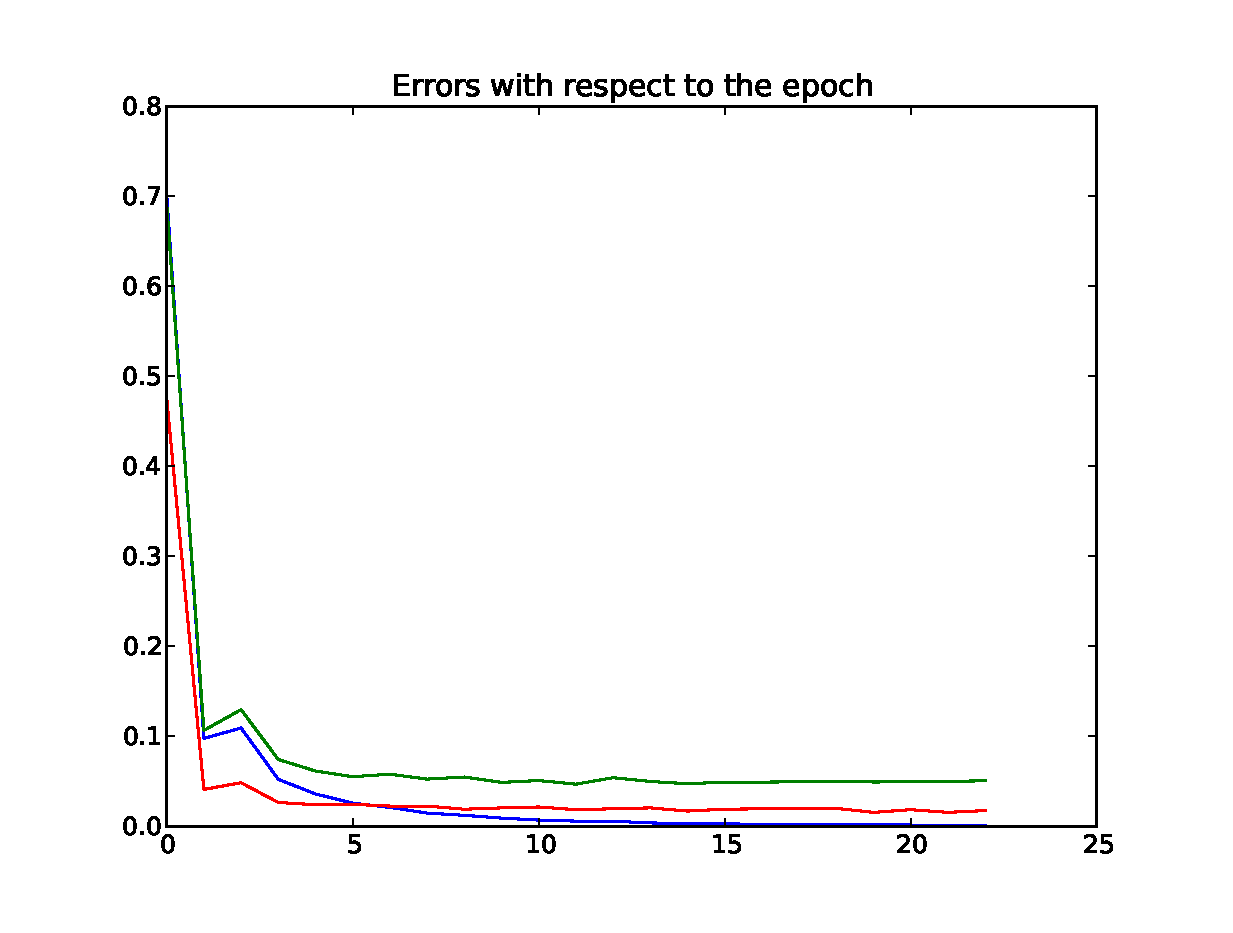
\includegraphics[width=0.3\textwidth]{../plots/learning_0.01__hidden_70.eps}}
    \subfloat[for $\eta = 0.01$  and $h_1 = 80$]{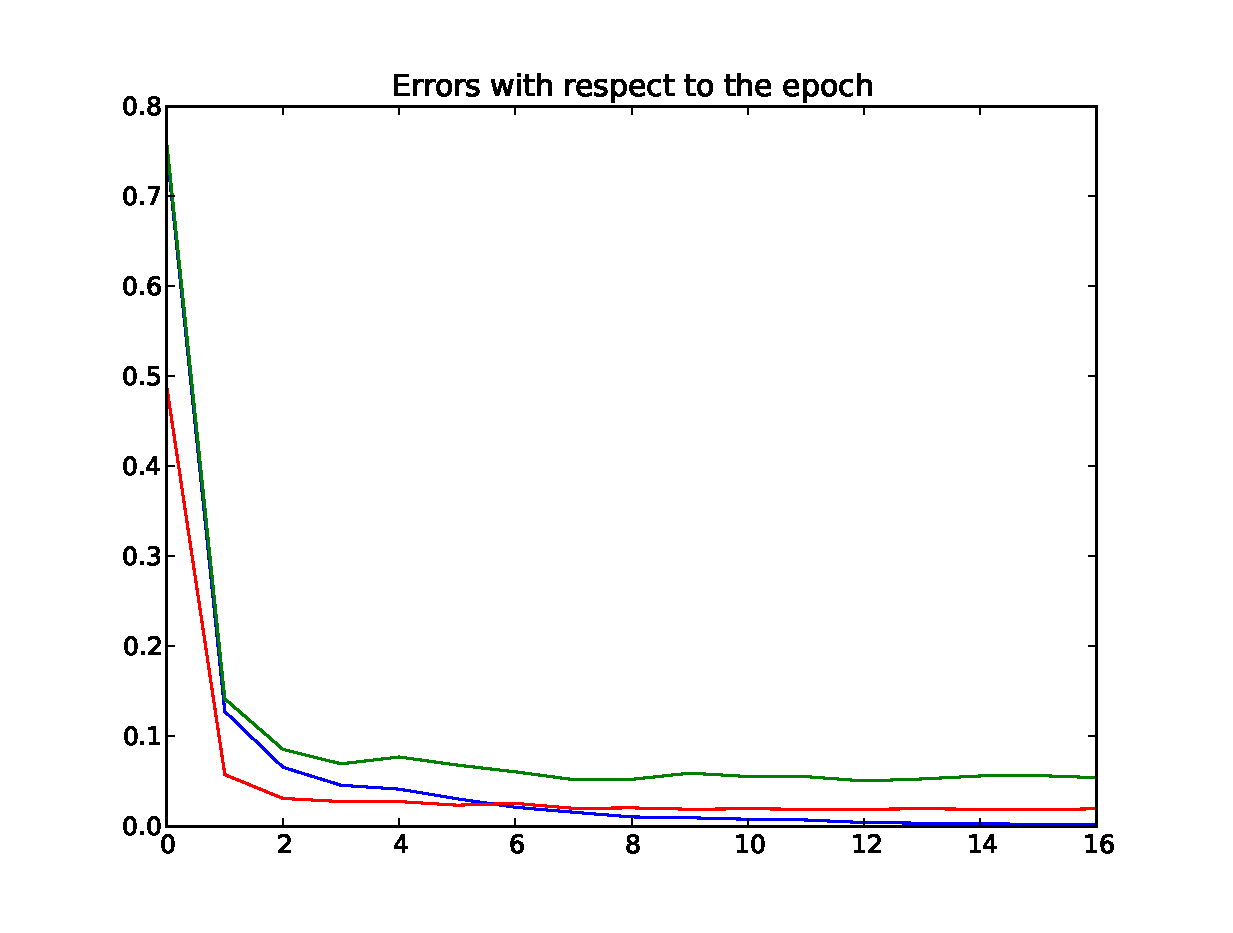
\includegraphics[width=0.3\textwidth]{../plots/learning_0.01__hidden_80.eps}}
    \subfloat[for $\eta = 0.01$  and $h_1 = 90$]{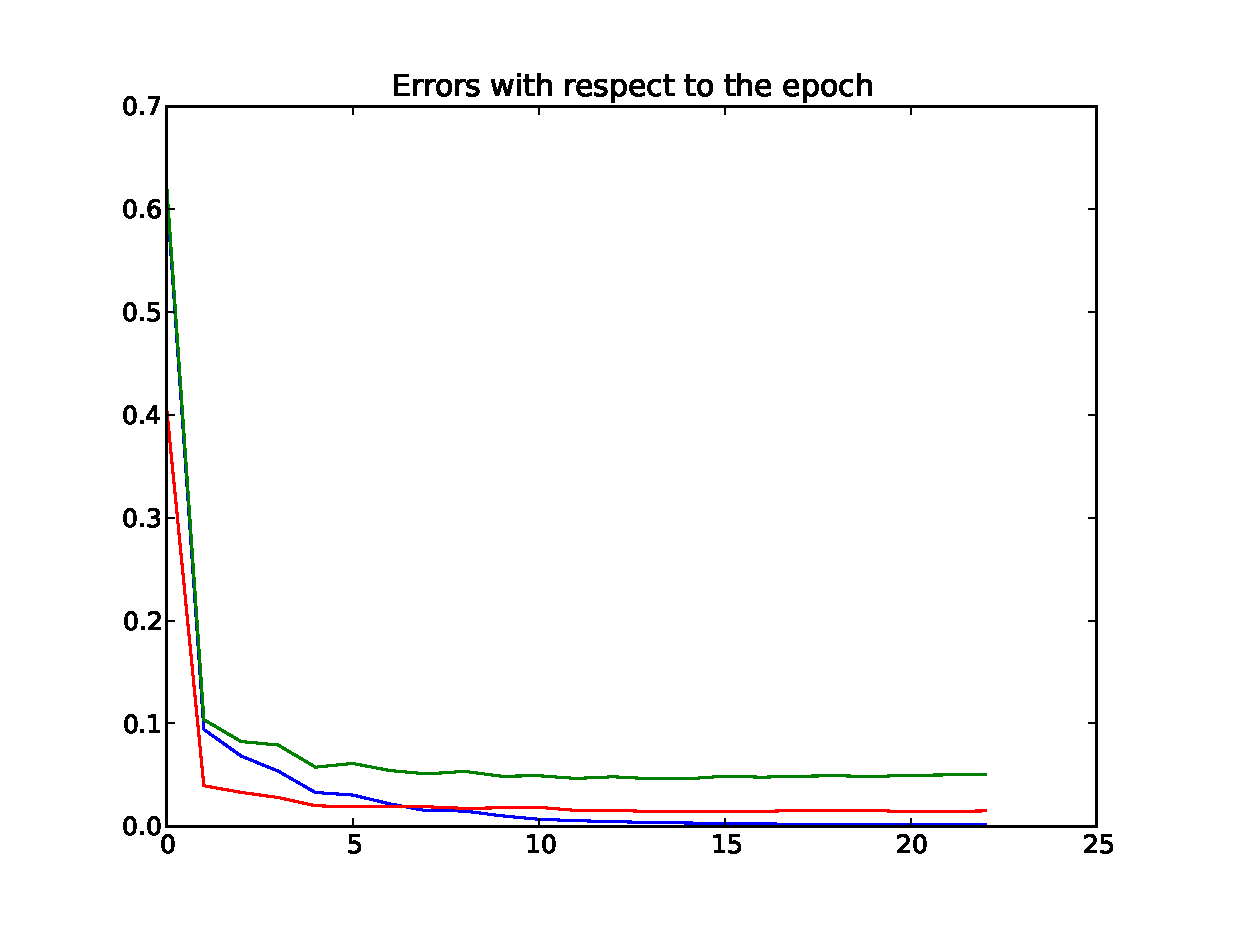
\includegraphics[width=0.3\textwidth]{../plots/learning_0.01__hidden_90.eps}}\\
    \subfloat[for $\eta = 0.01$  and $h_1 = 100$]{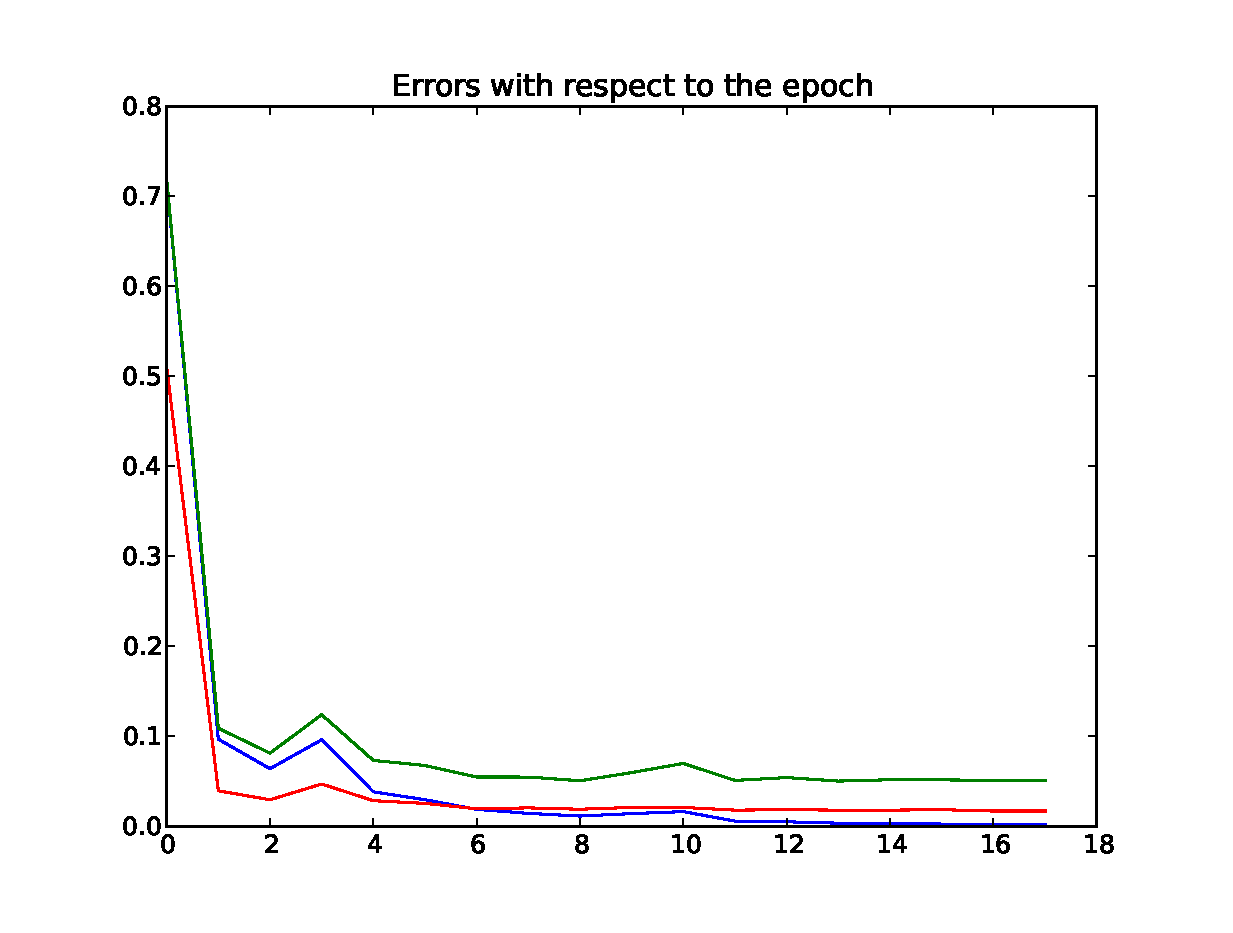
\includegraphics[width=0.3\textwidth]{../plots/learning_0.01__hidden_100.eps}}
    \caption{$E_{\mathrm{Log}}$ for training and validation set with 3-5 digits} 
    \label{fig:hidden}
\end{figure}

\begin{figure}[!h]
    \centering
    \subfloat[$h_1$ in function of the epoch number]{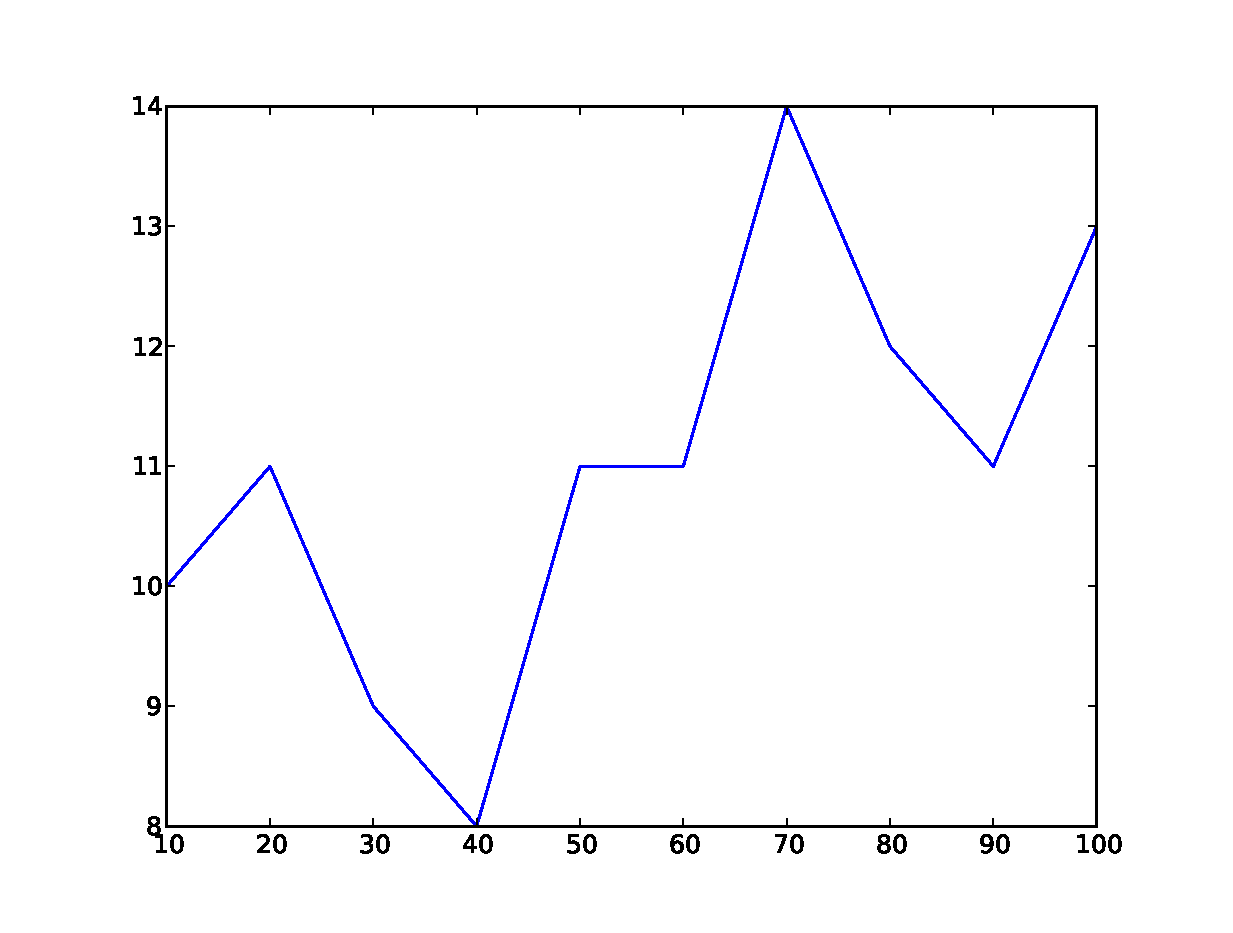
\includegraphics[width=0.5\textwidth]{../plots/plot_hidden_epoch_num}}
    \subfloat[$h_1$ in function of the error on the validation set]{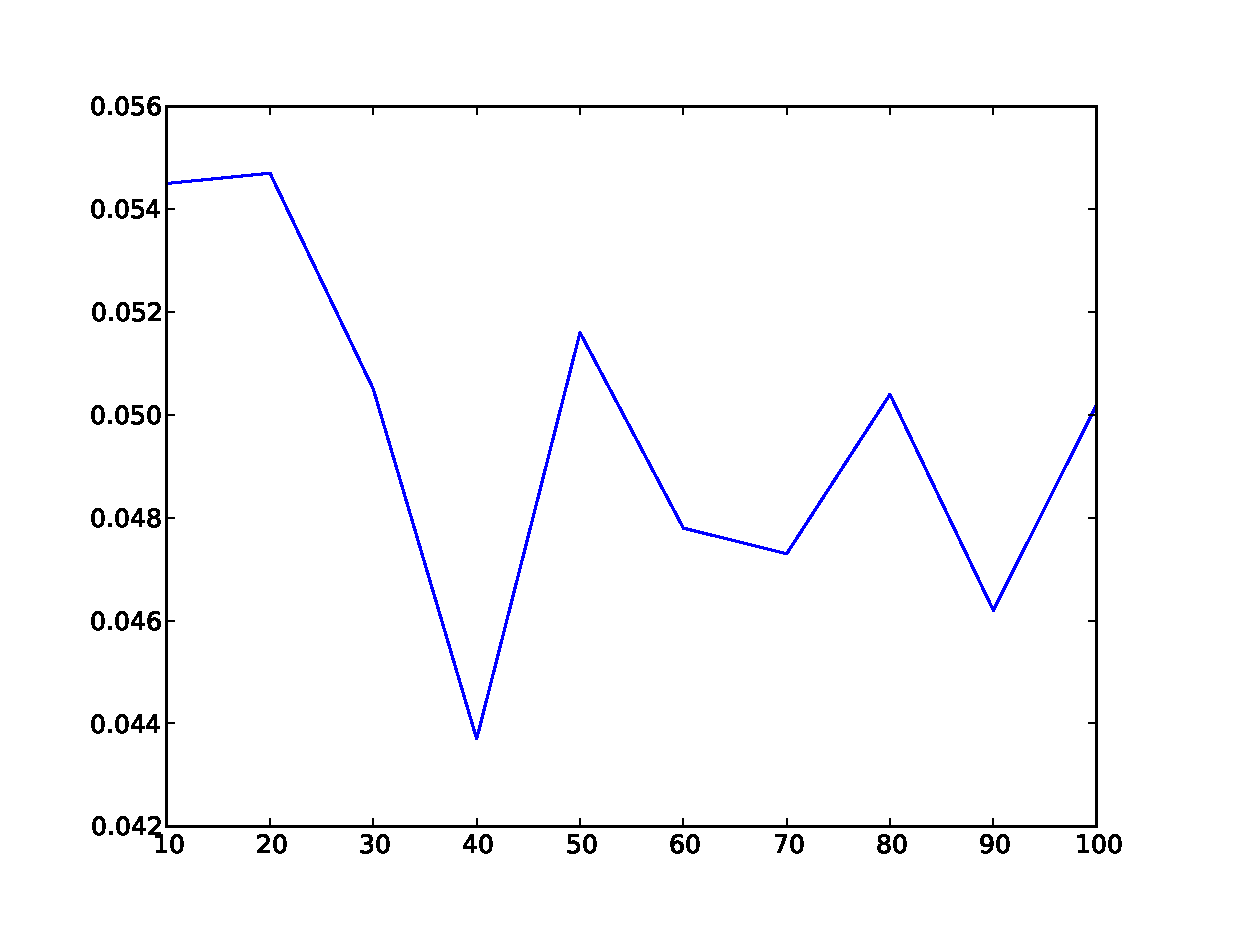
\includegraphics[width=0.5\textwidth]{../plots/plot_hidden_valid_error}}
    \caption{Comparative plots for $h_1$}
    \label{fig:comp-hidden}
\end{figure}
As can see in the plots, the more we have hidden units the more we have overfitting. On opposite with a too small value $h_1$, we do not have enough precision. Another remark we can do is that it also increases the epoch number. When $h_1$ increases, it also increases the computations time.
In the comparative plots of Figure~\ref{fig:comp-hidden}, we can see that the best value for $h_1$ is 40.

For the learning rate $\eta$ we tested values 0.1,0.01 and 0.001.
\begin{figure}[!h]
    \centering
    \subfloat[$\eta=0.1$]{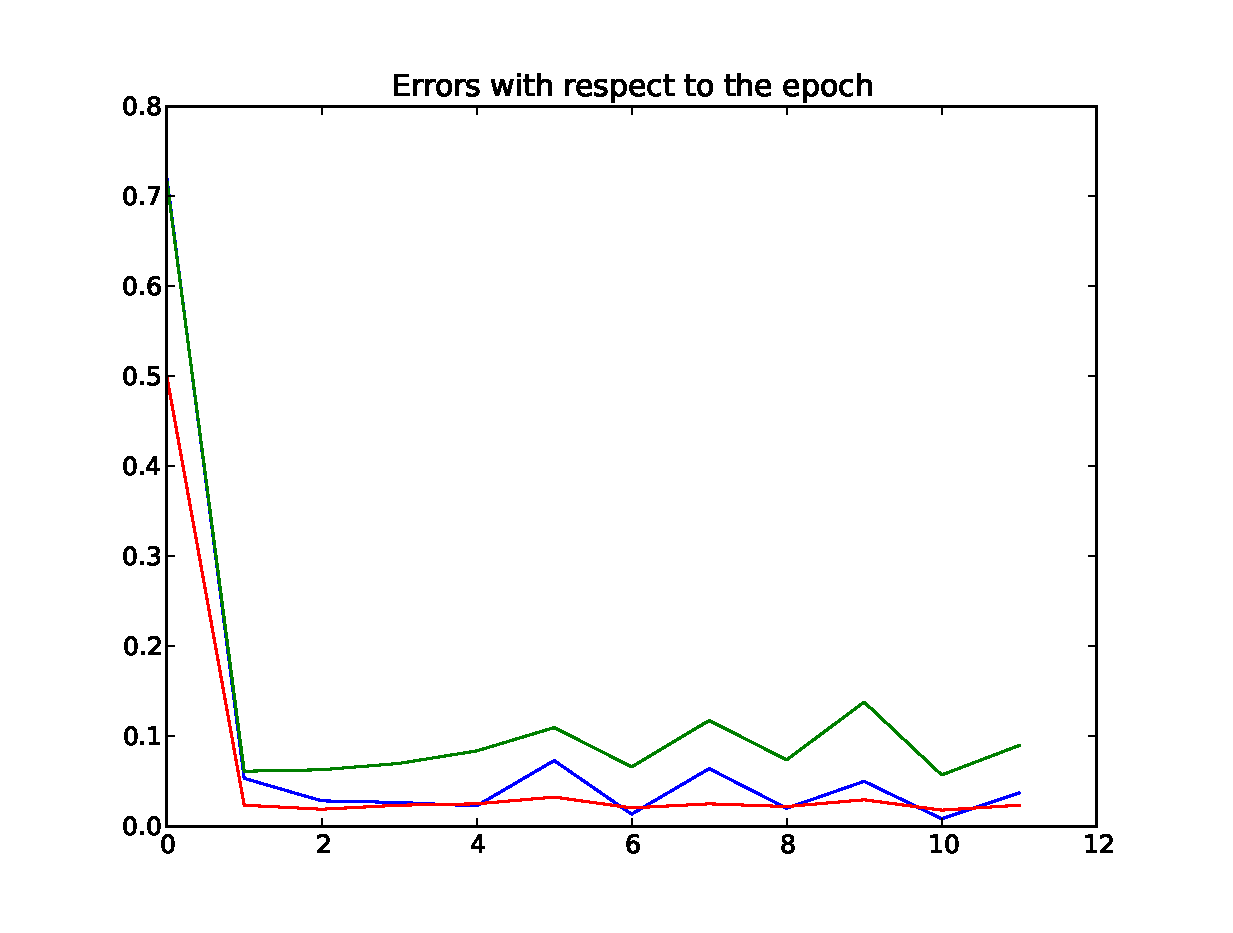
\includegraphics[width=0.3\textwidth]{../plots/learning_0.1__hidden_40__m_rate_0.5.eps}}
    \subfloat[$\eta=0.01$]{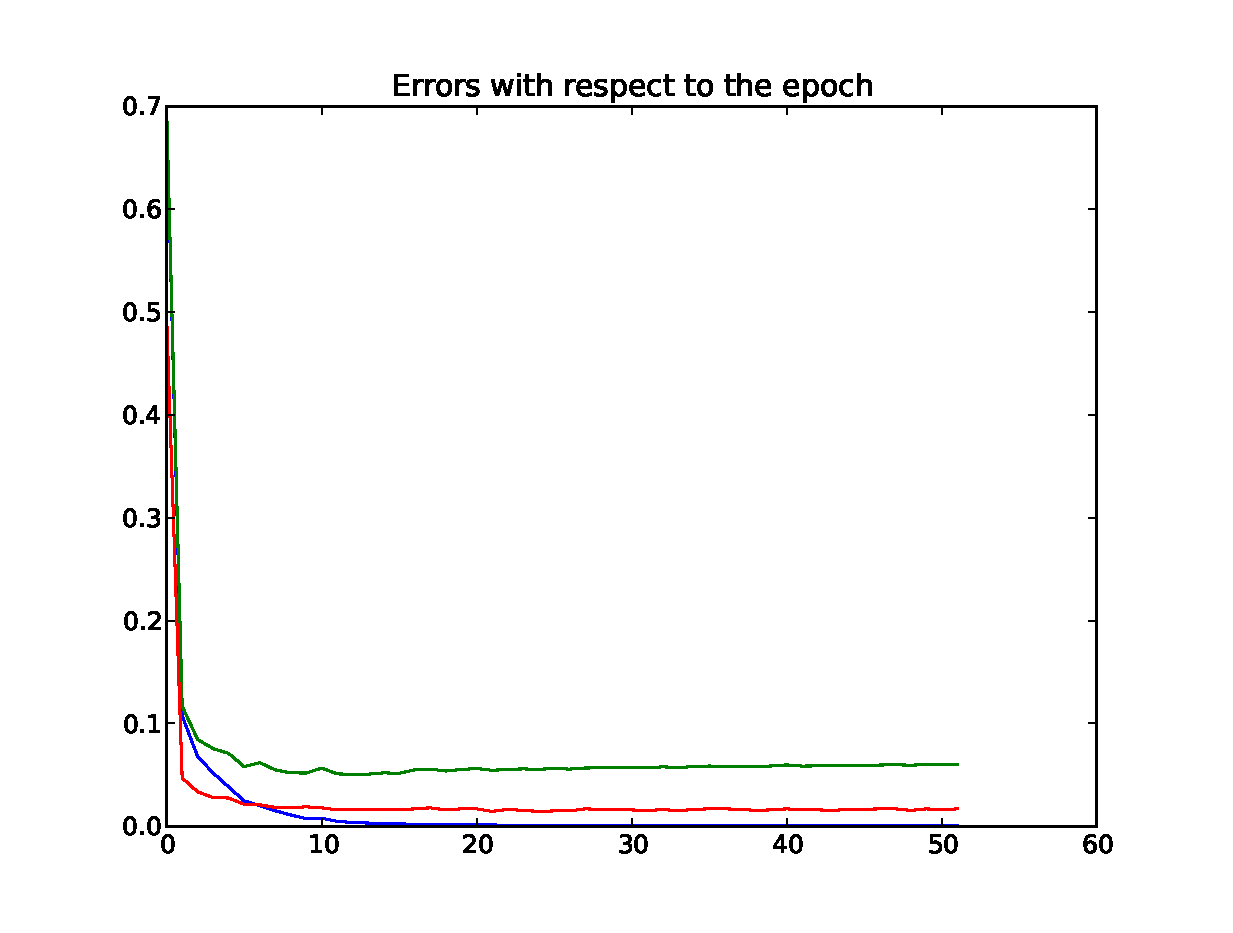
\includegraphics[width=0.3\textwidth]{../plots/learning_0.01__hidden_40__m_rate_0.5.eps}}
    \subfloat[$\eta=0.001$]{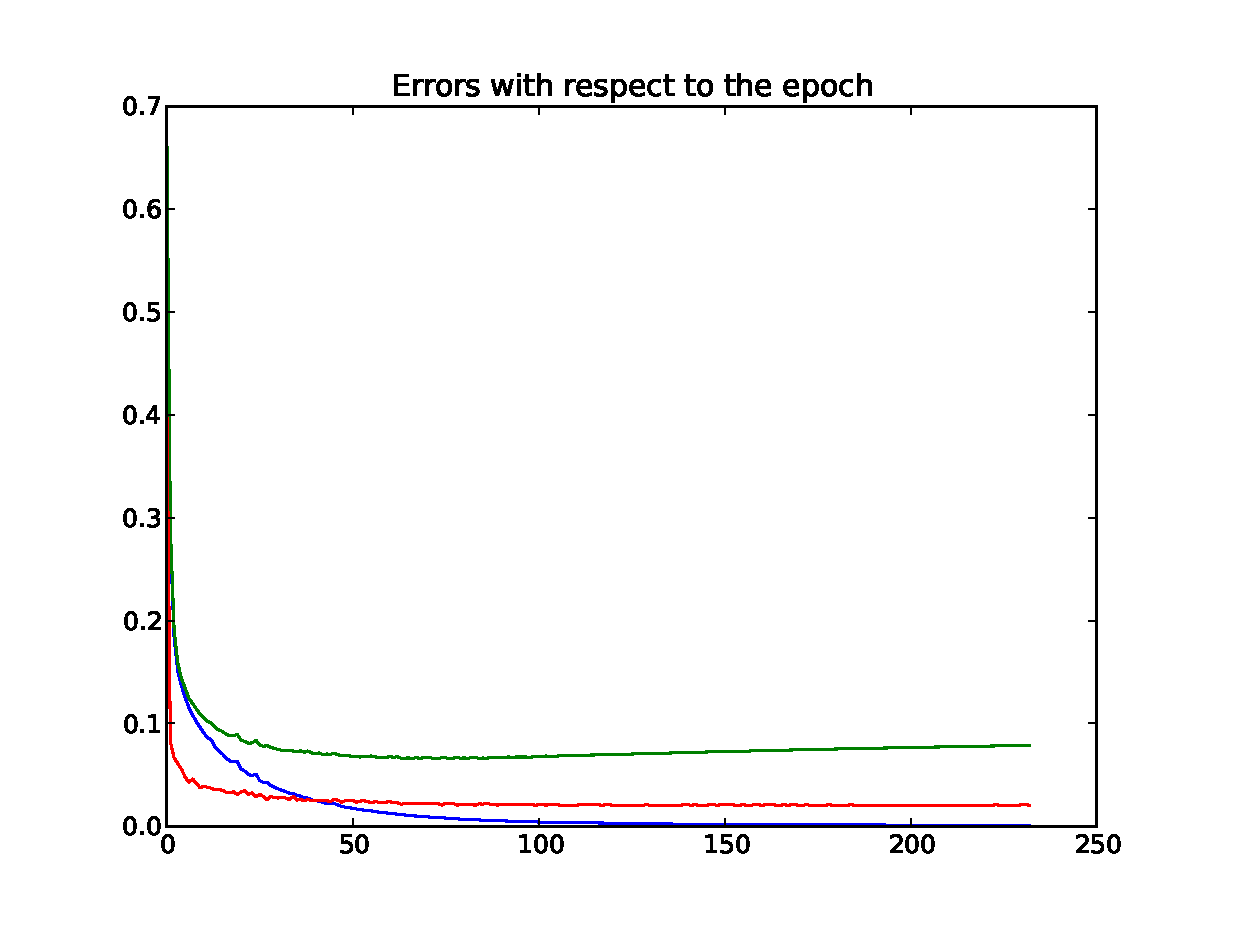
\includegraphics[width=0.3\textwidth]{../plots/learning_0.001__hidden_40__m_rate_0.5.eps}}
\end{figure}
For the plots, we notice that too small learning rates lead to very slow convergence i.e. the epoch number increases drastically.  
For example between 0.01 and 0.001 the convergence speed is very different. For $\eta=0.1$ the convergence is not clear and it zigzags.
Consequently we decided to take $\eta = 0.01$.

For the momentum rate $\mu$ we tested values 0.1,0.2,...,0.9. 
\begin{figure}[!h]
    \centering
    \subfloat[for $\eta = 0.01$  ,$h_1 = 40$ ,$\mu = 0.1$]{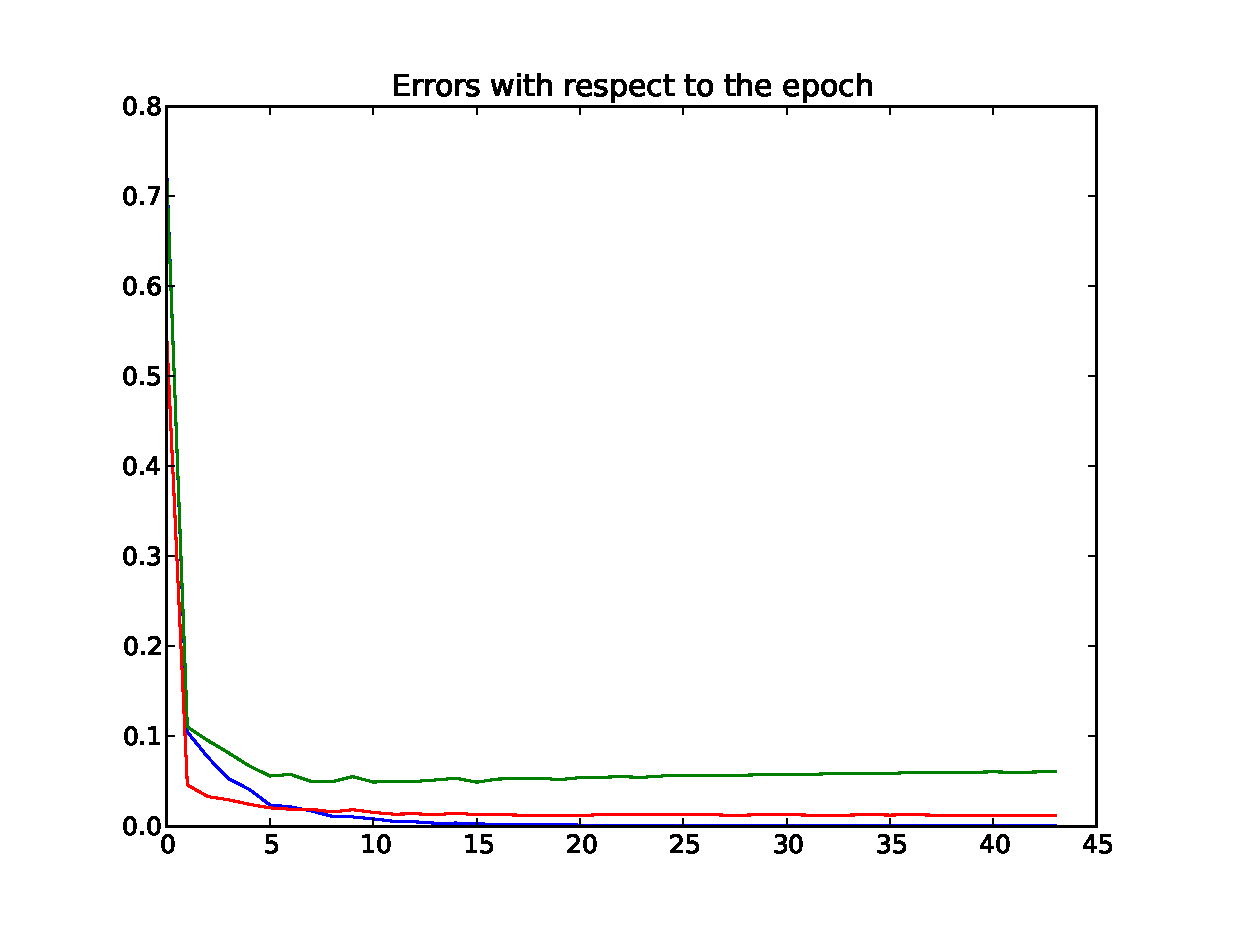
\includegraphics[width=0.3\textwidth]{../plots/learning_0.01__hidden_40__m_rate_0.1.eps}}
    \subfloat[for $\eta = 0.01$  ,$h_1 = 40$ ,$\mu = 0.2$]{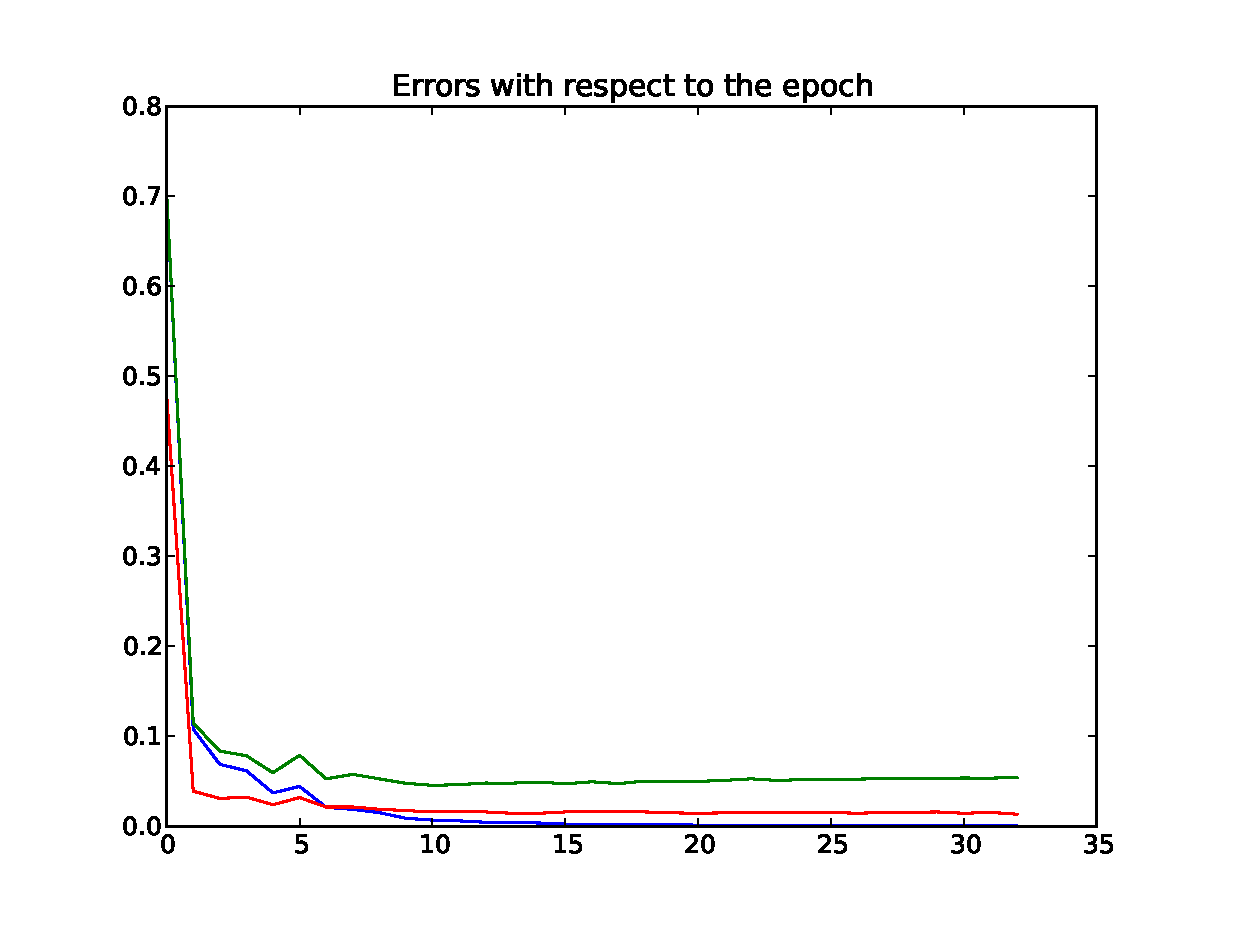
\includegraphics[width=0.3\textwidth]{../plots/learning_0.01__hidden_40__m_rate_0.2.eps}}
    \subfloat[for $\eta = 0.01$  ,$h_1 = 40$ ,$\mu = 0.3$]{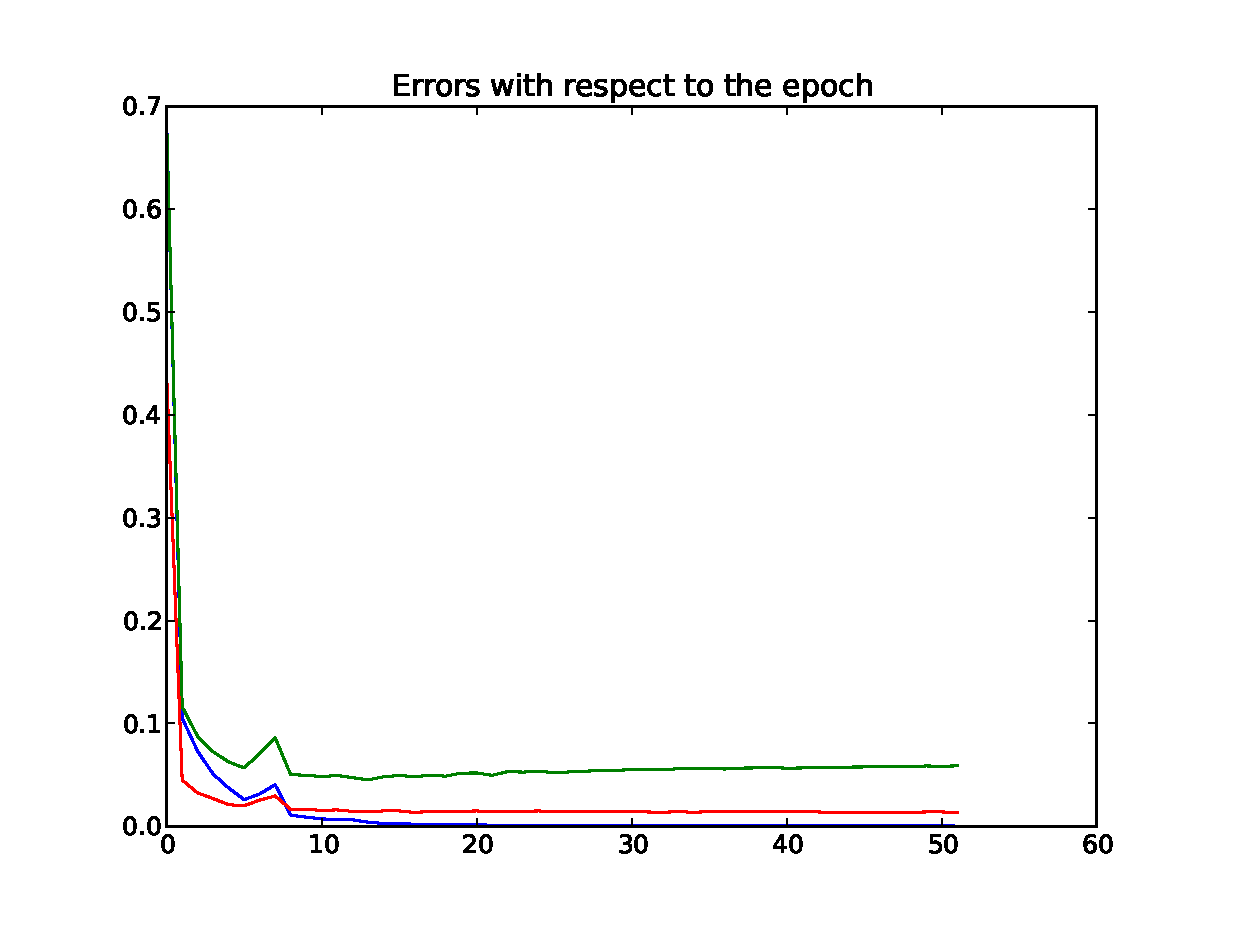
\includegraphics[width=0.3\textwidth]{../plots/learning_0.01__hidden_40__m_rate_0.3.eps}}\\
    \subfloat[for $\eta = 0.01$  ,$h_1 = 40$ ,$\mu = 0.4$]{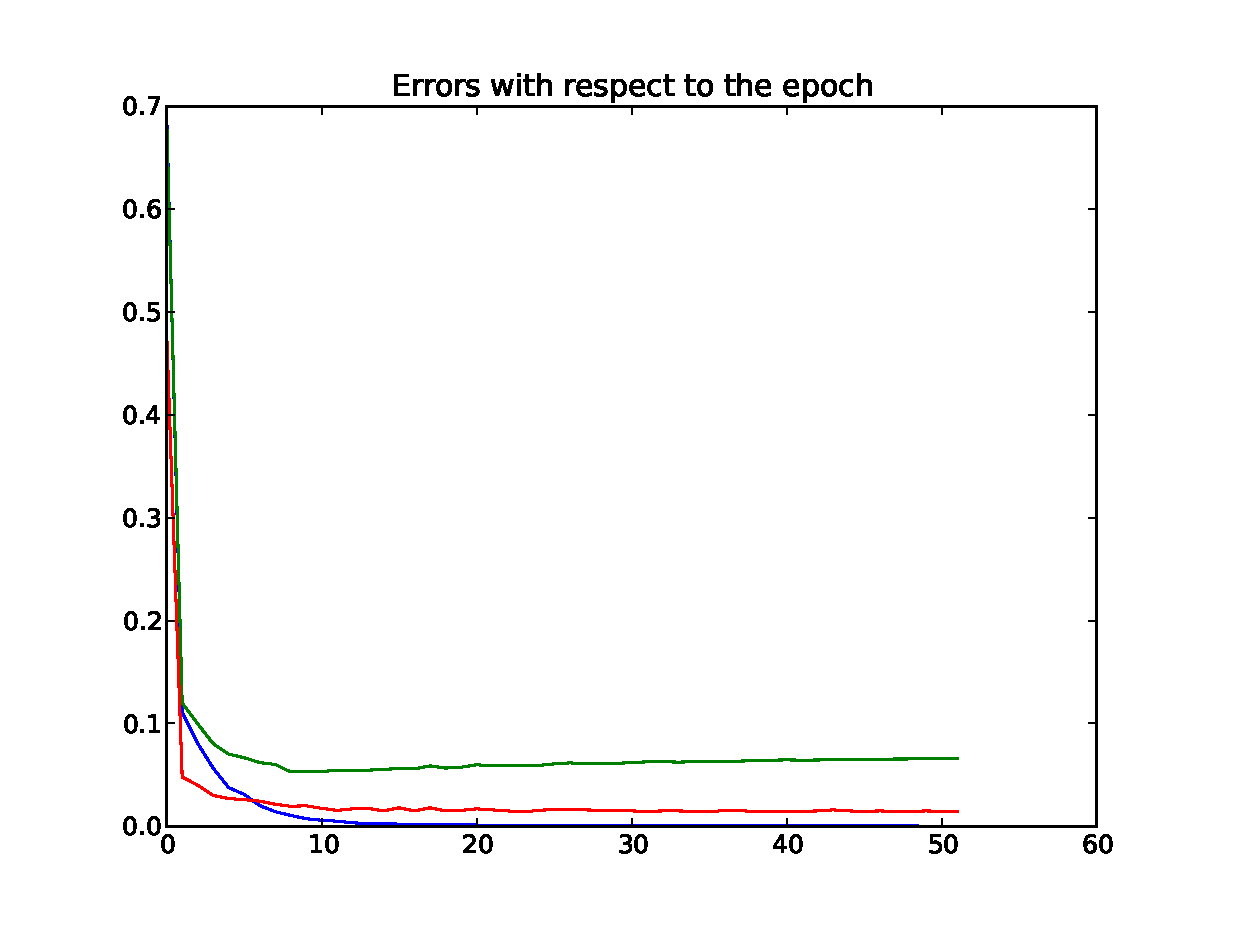
\includegraphics[width=0.3\textwidth]{../plots/learning_0.01__hidden_40__m_rate_0.4.eps}}
    \subfloat[for $\eta = 0.01$  ,$h_1 = 40$ ,$\mu = 0.5$]{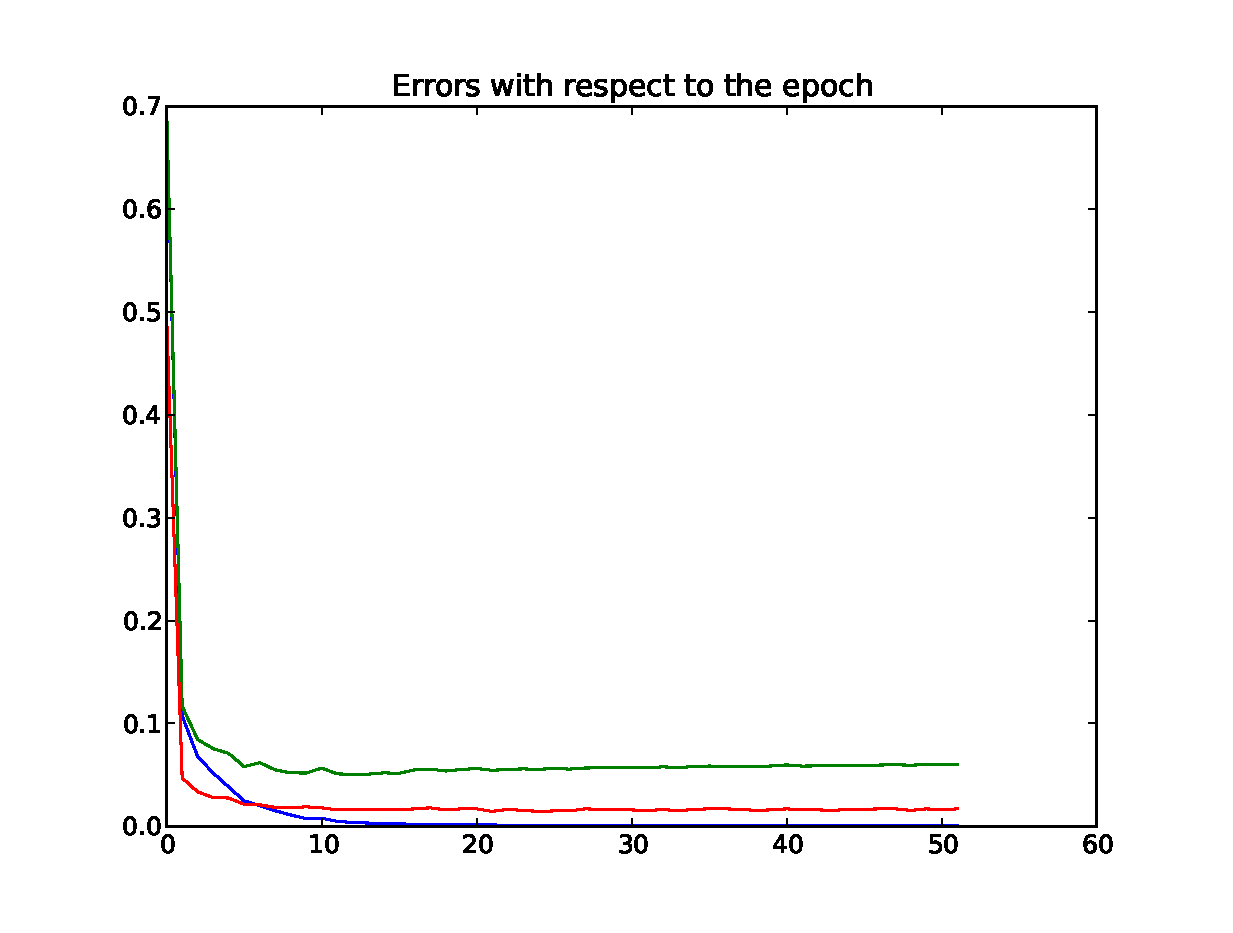
\includegraphics[width=0.3\textwidth]{../plots/learning_0.01__hidden_40__m_rate_0.5.eps}}
    \subfloat[for $\eta = 0.01$  ,$h_1 = 40$ ,$\mu = 0.6$]{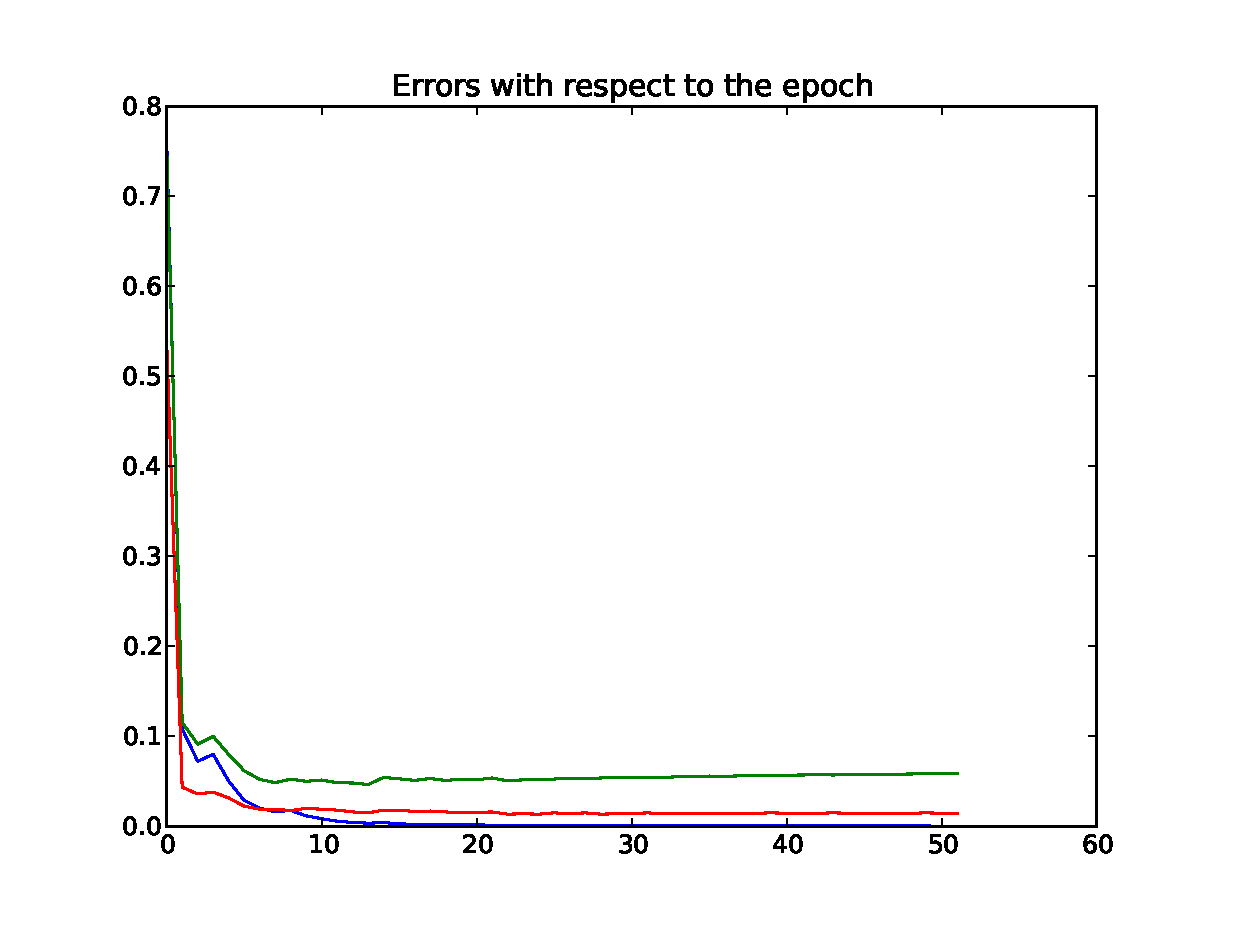
\includegraphics[width=0.3\textwidth]{../plots/learning_0.01__hidden_40__m_rate_0.6.eps}}\\
    \subfloat[for $\eta = 0.01$  ,$h_1 = 40$ ,$\mu = 0.7$]{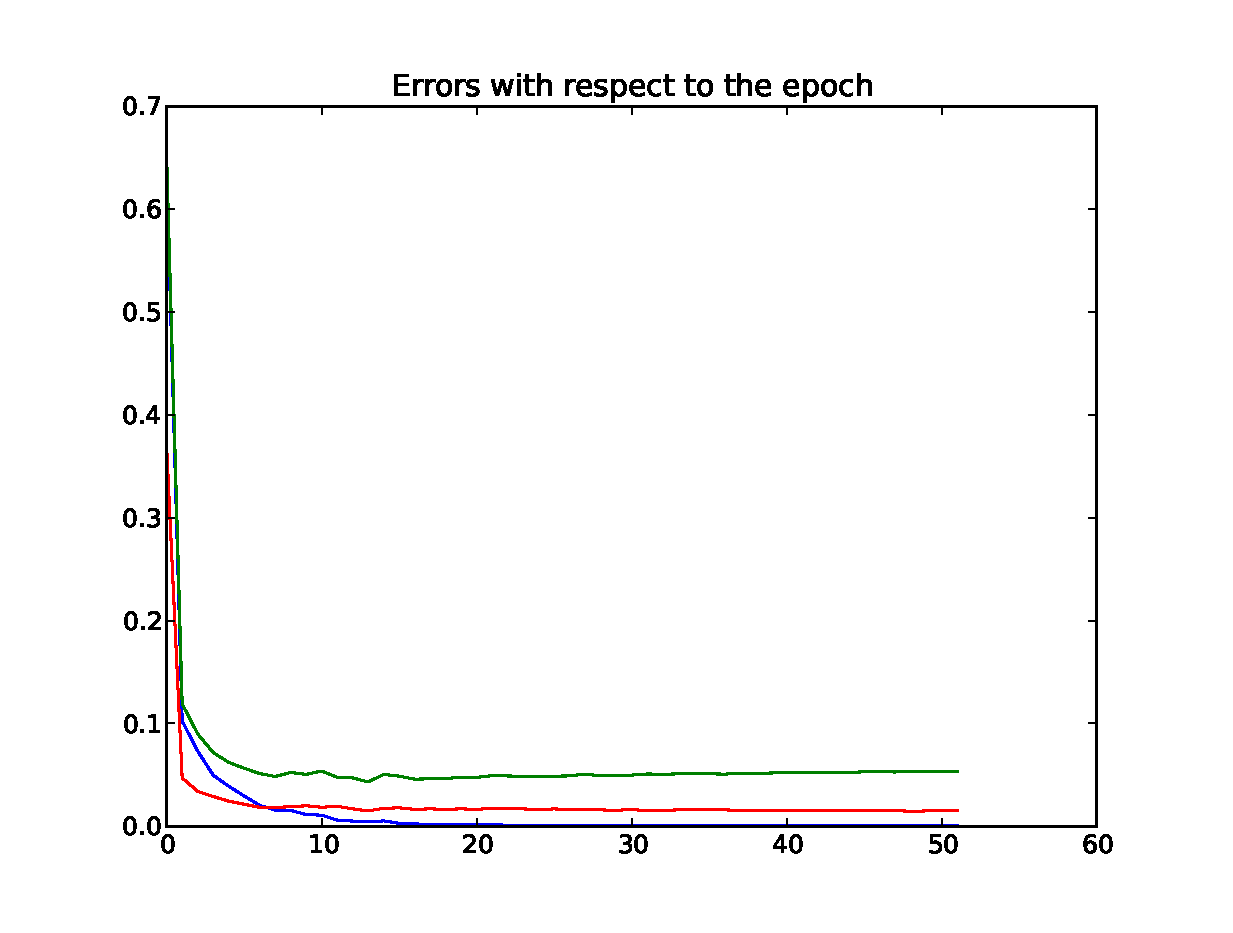
\includegraphics[width=0.3\textwidth]{../plots/learning_0.01__hidden_40__m_rate_0.7.eps}}
    \subfloat[for $\eta = 0.01$  ,$h_1 = 40$ ,$\mu = 0.8$]{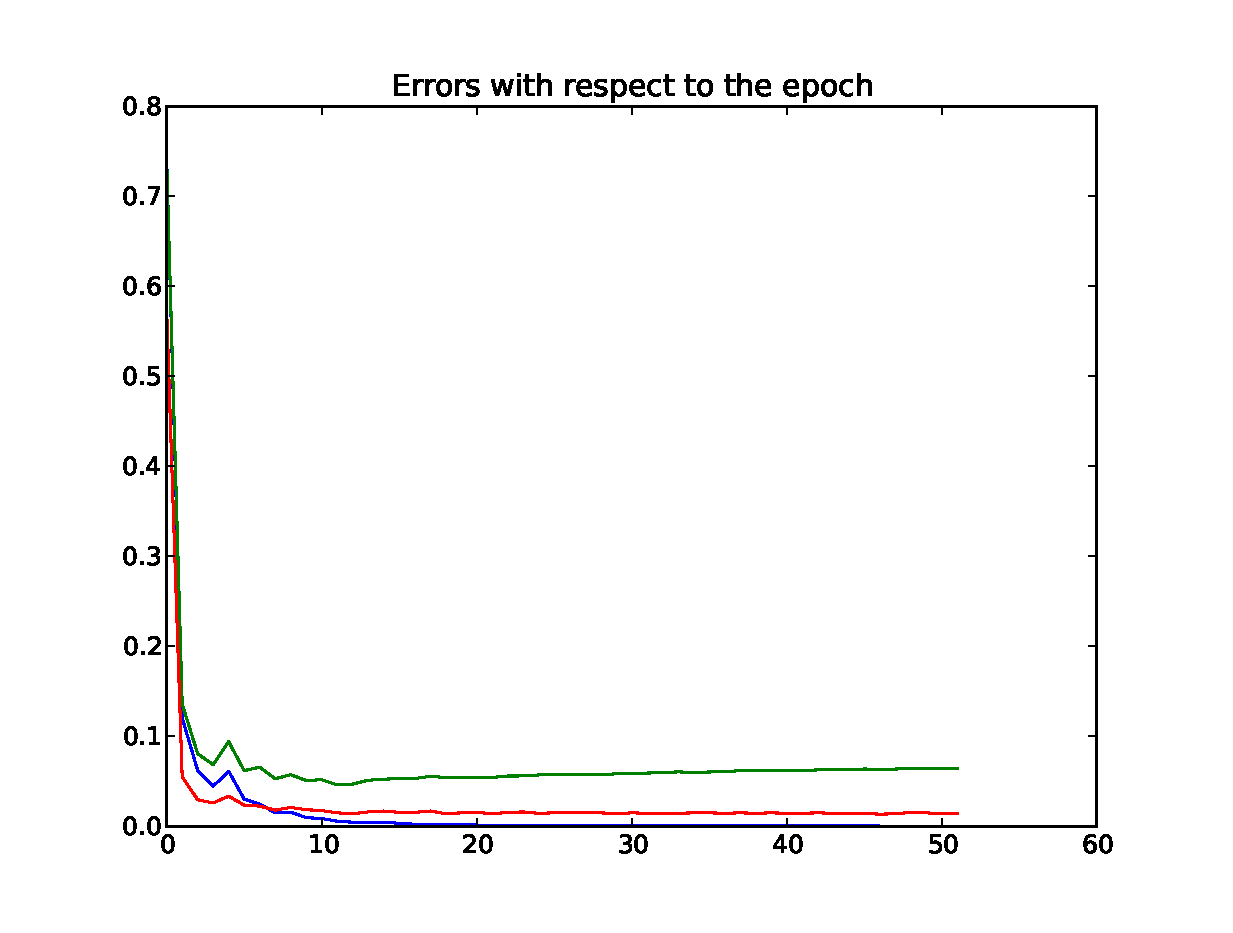
\includegraphics[width=0.3\textwidth]{../plots/learning_0.01__hidden_40__m_rate_0.8.eps}}
    \subfloat[for $\eta = 0.01$  ,$h_1 = 40$ ,$\mu = 0.9$]{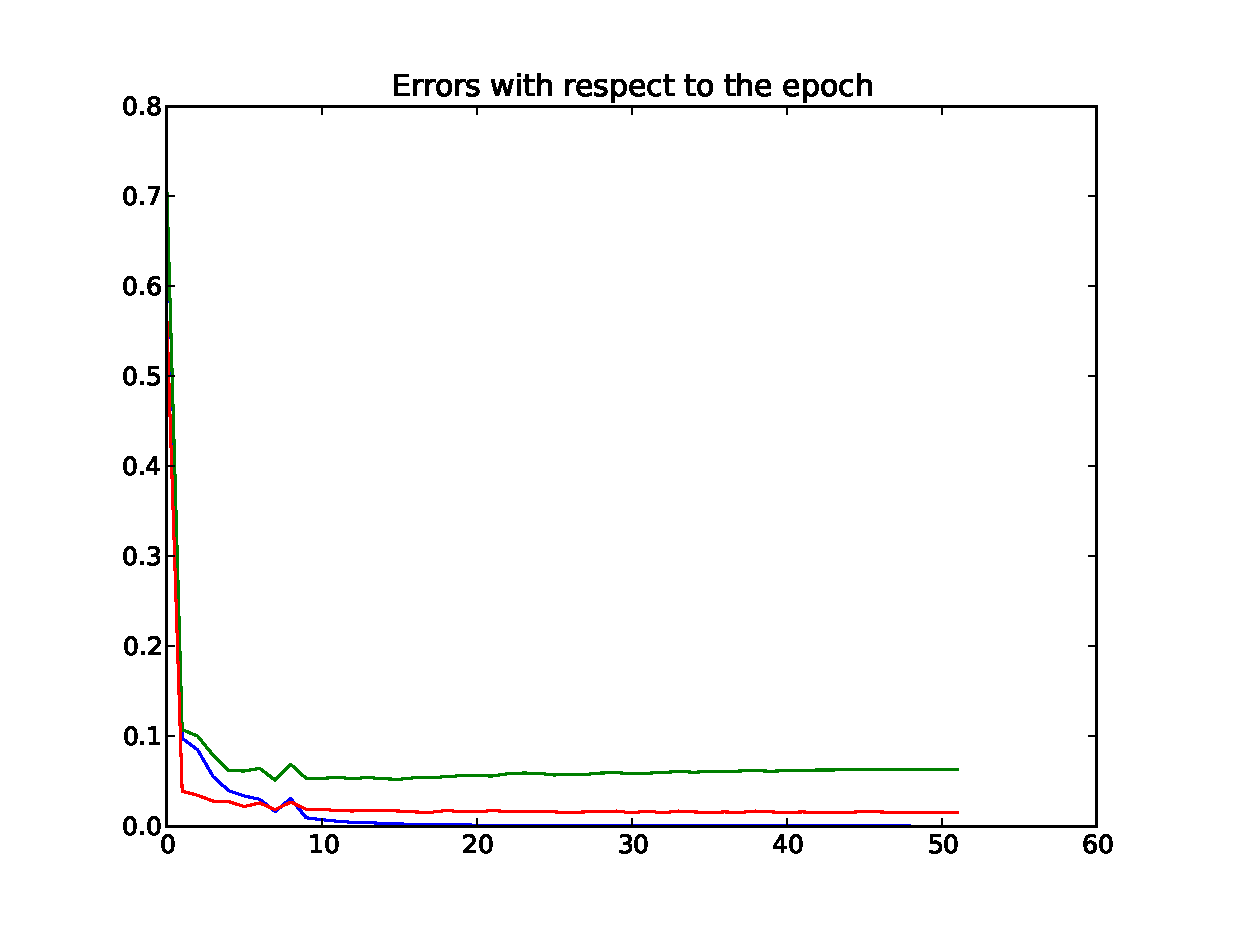
\includegraphics[width=0.3\textwidth]{../plots/learning_0.01__hidden_40__m_rate_0.9.eps}}
    \caption{$E_{\mathrm{Log}}$ for training and validation set with 3-5 digits} 
    \label{fig:mu}
\end{figure}
And it is very difficult to deduce something from the plots.


For both binary tasks we chose $\eta = 0.01$, $\mu = 0.5$ and $h_1 = 40$. They seemed to be the best even if it was difficult to decide.

\subsection*{Results and Discussion}

On the 3-5 discrimination problem, we have a success rate of 0.986. This is what we expected. For the 4-9 discrimination, it is about the same. It is 0.977.\\*
By setting appropriate values for the various constants as we have previously seen, we can achieve a good success rate with a reasonable number of epochs. However, there is obviously not a 100\% success rate, but as one can si below in Figure~\ref{fig:wrongclass} the digits have to be significantly distorted in order for the classification to fail.

\begin{figure}[!h]
    \centering
    \subfloat[It is a 5 but the classification slightly mistook it for a 3]{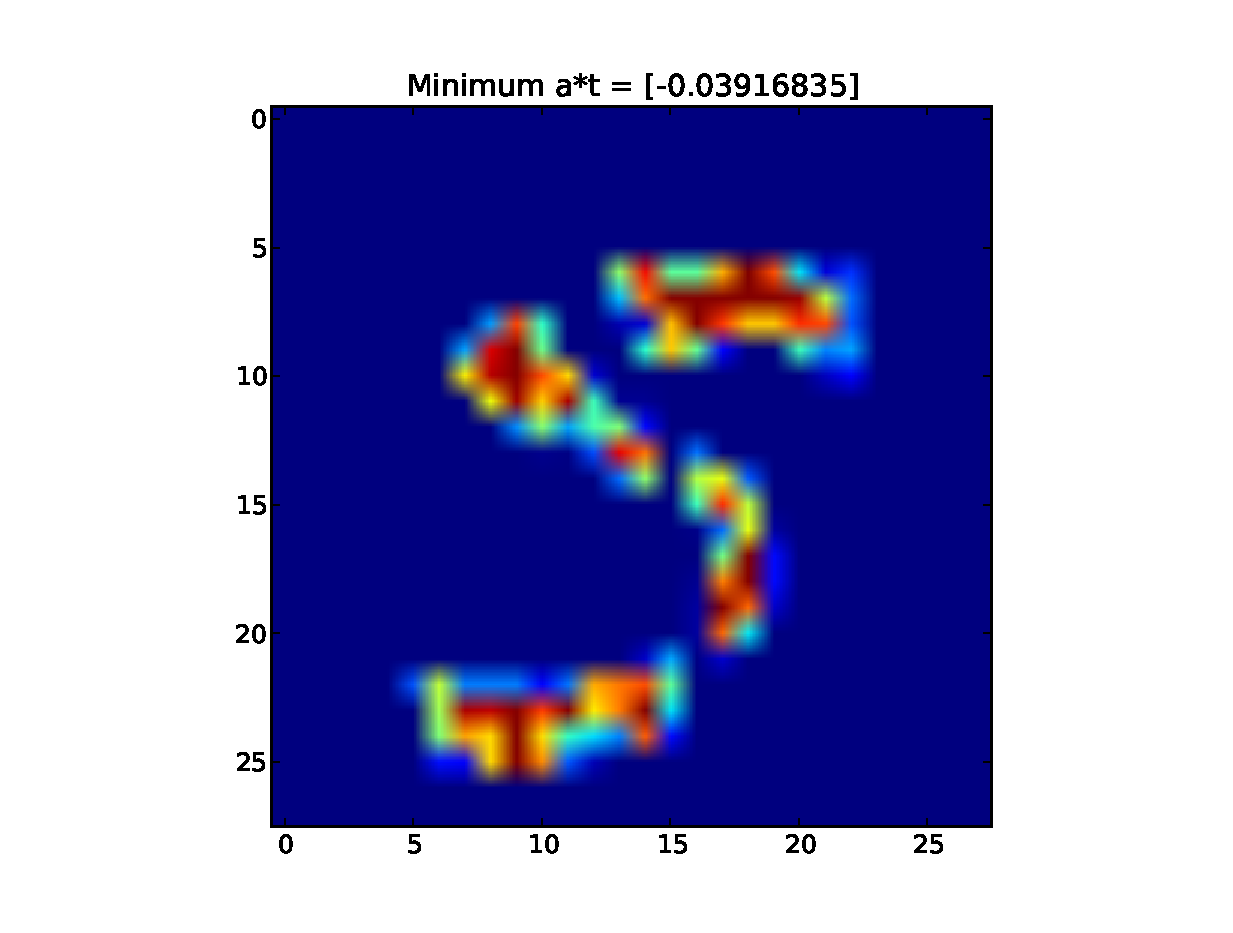
\includegraphics[width=0.3\textwidth]{../plots/min.eps}}
    \subfloat[5 that has been the most mistaken for a 3]{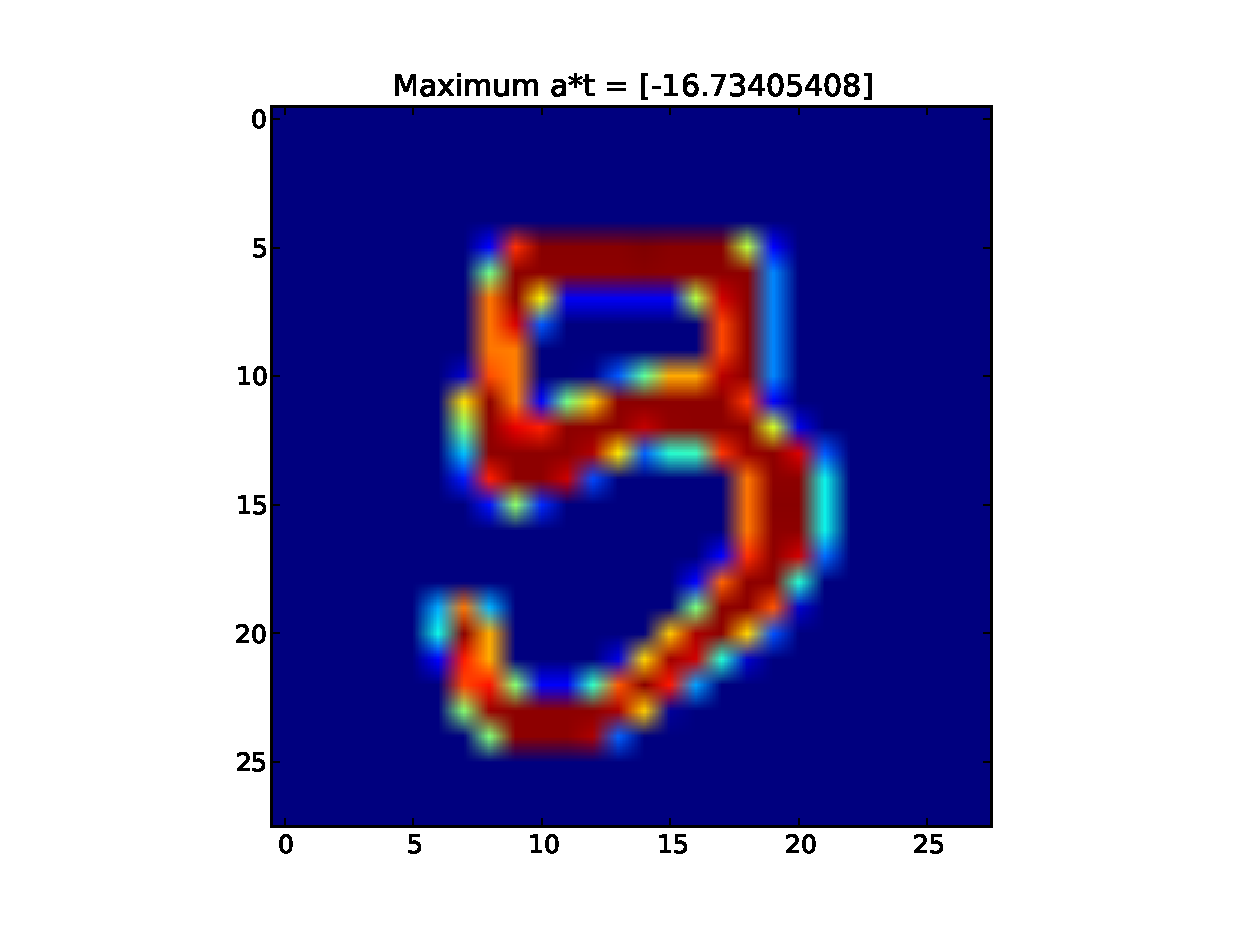
\includegraphics[width=0.3\textwidth]{../plots/max.eps}}
    \caption{Wrong classification} 
    \label{fig:wrongclass}
\end{figure}

As we see in this plot, although a human can still distinguish the characters, it is understandable that the classification fails.

\section*{Support Vector Machines}

\subsection*{Splitting and Preprocessing}

We do cross-validation, that is we split the sample vectors in $ n $ sets and then run $ n $ times the SVM algorithm each time with a different set as a validation set.\\*
The preprocessing is exactly the same as with the multi-layer perceptron.

\subsection*{SVM Setup}

To solve SVM, we implemented SMO. There are two parameters to learn to be chosen, namely $C$ and $\tau$. These parameters are obtained by running a
10-fold cross-validation on the training set. The training set contains 6000 data elements. Therefore for each cross-validation step, we train on 5400
and evaluate on 600 data elements. See in Figure~\ref{fig:paramtab} the table with all the results we got with the cross-validation. 
This table allows us to choose the best parameters for SVM. We variated parameters $C$ and $\tau$ the following way. For each of them, we tried with values
$2^{-5} , 2^{-4} , ... , 2^{3},2^{4}$.

\subsection*{Results and Discussion}
In order to tweak $ C $ and $ \tau $, we had to run several instances of SVM, each time with different parameters.
As it would take too much time on a laptop, we decided to distribute the computation on 50 workstations\footnote{We used the machines in BC07 each running two instances of SVM with different probabilities.}. Each one had to run the same algorithm twice with a different set of values for $ C $ and $ \tau $ thus allowing us to complete the following table:xs

\begin{figure}[!h]
\centering
\begin{tabular}{|l|l|l|l|l|l|l|l|l|l|l|}
    \hline
    \diagbox[height=38pt,width=38pt]{$\log\tau$} {$\log C$} & -5   & -4   & -3   & -2   & -1   & 0    & 1    & 2    & 3    & 4 \\ \hline
    -5                  &0.0311&\textbf{0.0050}&0.0056&0.0065&0.0075&0.0089&0.0118&0.0146&0.0166&0.0166 \\ \hline
    -4                  &0.0064&0.0068&0.0070&0.0071&0.0080&0.0095&0.0111&0.0122&0.0122&0.0122 \\ \hline
    -3                  &0.0152&0.0202&0.0237&0.0257&0.0267&0.0287&0.0300&0.0301&0.0301&0.0301 \\ \hline
    -2                  &0.0284&0.0513&0.0847&0.1281&0.1800&0.2130&0.2158&0.2158&0.2158&0.2158 \\ \hline
    -1                  &0.0310&0.0617&0.1224&0.2406&0.4641&0.8009&0.8088&0.8088&0.8088&0.8088 \\ \hline
     0                  &0.0311&0.0622&0.1245&0.2489&0.4975&0.9920&0.9940&0.9940&0.9940&0.9940 \\ \hline
     1                  &0.0311&\textbf{0.0050}&0.1245&0.0065&0.4982&0.0089&0.0118&0.0146&0.0166&0.9999 \\ \hline
     2                  &0.0311&0.0622&0.1245&0.0071&0.0080&0.0095&0.0111&0.0122&0.9999&0.9999 \\ \hline
     3                  &0.0311&0.0622&0.1245&0.0257&0.4982&0.0287&0.0300&0.0301&0.0122&0.0301 \\ \hline
     4                  &0.0311&0.0622&0.1245&0.1281&0.1800&0.9965&0.2158&0.2158&0.2158&0.2158 \\ \hline
\end{tabular}
\caption{Parameter table}
\label{fig:paramtab}
\end{figure}

The best values (i.e. lowest risk) are in bold. Thus we choose the values $ C = 2^{-4} $ and $ \tau = 2^{-5} $.

When running svm on the test set we got an error of 0.026.
\section*{Conclusion}

The SVM implementation is much simpler and it is easier to see what happens at each step of the computation. MLP on the other hand is conceptually easier to understand as it is a natural evolution of the Perceptron algorithm. Moreover
it is faster in computation time than SVM.
The project in general was worth the effort. We now see a little better the potential of these techniques and how powerful they could be. As they are sufficiently general to be applied to a wide range of other problems, we can easily apply the skills acquired in this project to other situations.

\end{document}
